\documentclass{beamer}

\usepackage{amssymb,amsmath}
\usepackage{graphicx}
\usepackage{url}
\usepackage{color}
\usepackage{pagenote}[continuous,page]
\usepackage{relsize}		% For \smaller
\usepackage{url}			% For \url
\usepackage{epstopdf}	% Included EPS files automatically converted to PDF to include with pdflatex

%For MindMaps
% \usepackage{tikz}%
% \usetikzlibrary{mindmap,trees,arrows}%

%%% Color Definitions %%%%%%%%%%%%%%%%%%%%%%%%%%%%%%%%%%%%%%%%%%%%%%%%%%%%%%%%%
%\definecolor{bordercol}{RGB}{40,40,40}
%\definecolor{headercol1}{RGB}{186,215,230}
%\definecolor{headercol2}{RGB}{80,80,80}
%\definecolor{headerfontcol}{RGB}{0,0,0}
%\definecolor{boxcolor}{RGB}{186,215,230}

%%% Save space in lists. Use this after the opening of the list %%%%%%%%%%%%%%%%
%\newcommand{\compresslist}{
%	\setlength{\itemsep}{1pt}
%	\setlength{\parskip}{0pt}
%	\setlength{\parsep}{0pt}
%}

%\setbeameroption{show notes on top}

% You should run 'pdflatex' TWICE, because of TOC issues.

% Rename this file.  A common temptation for first-time slide makers
% is to name it something like ``my_talk.tex'' or
% ``john_doe_talk.tex'' or even ``discrete_math_seminar_talk.tex''.
% You really won't like any of these titles the second time you give a
% talk.  Try naming your tex file something more descriptive, like
% ``riemann_hypothesis_short_proof_talk.tex''.  Even better (in case
% you recycle 99% of a talk, but still want to change a little, and
% retain copies of each), how about
% ``riemann_hypothesis_short_proof_MIT-Colloquium.2000-01-01.tex''?

\mode<presentation>
{
  \usetheme{CambridgeUS}		% bem bacana - menu superior
  \usecolortheme{default}		% branco, azul clarinho
  \useoutertheme{default}
  \useinnertheme{circles}
  \setbeamercovered{invisible}
}

\beamertemplatenavigationsymbolsempty

%% Better looking blocks
\setbeamercolor{block title alerted}{use=structure,fg=black,bg=red!80!black}
\setbeamercolor{block body alerted}{use=structure,fg=black,bg=white!90!black}

\setbeamercolor{block title}{use=structure,fg=black,bg=blue!60!white}
\setbeamercolor{block body}{use=structure,fg=black,bg=white!90!black}

\usepackage[english]{babel}
\usepackage[latin1]{inputenc}
\usepackage{subfigure}

\usepackage{times}
\usepackage[T1]{fontenc}

%% makes the ppagenote command for figure references at the end.
\makepagenote
\renewcommand{\notenumintext}[1]{}
\newcommand{\ppagenote}[1]{\pagenote[Page \insertframenumber]{#1}}


\usepackage{tikz}
\usetikzlibrary{arrows,shapes}

\title[GB13604]{GB13604 - Maths for Computer Science}
\subtitle[]{Lecture 4 -- Graphs Part I}
\author[Claus Aranha]{Claus Aranha\\{\footnotesize caranha@cs.tsukuba.ac.jp}}
\institute[COINS]{College of Information Science}
\date[2018-10-24]{2018-10-24\\{\tiny Last updated \today}}

\tikzstyle{vertex}=[circle,fill=black!25,minimum size=10pt,inner sep=0pt]
\tikzstyle{blue vertex}=[circle,fill=blue!100,minimum size=10pt,inner sep=0pt]
\tikzstyle{red vertex}=[circle,fill=red!100,minimum size=10pt,inner sep=0pt]
\tikzstyle{edge} = [draw,thick,-]
\tikzstyle{pedge} = [draw,thick,.]
\tikzstyle{red edge} = [draw, thick,-,red!50]
\tikzstyle{black edge} = [draw, line width=2pt,-,black!20]
\tikzstyle{weight} = [font=\smaller]

\begin{document}

\begin{frame}
  \maketitle

  \begin{center}
    {\smaller This course is based on Mathematics for Computer Science, Spring
    2015, by Albert Meyer and Adam Chlipala, Massachusetts Institute
    of Technology OpenCourseWare.}

    
\includegraphics[width=0.2\textwidth]{../img/by-nc-sa}
  \end{center}
\end{frame}

\section{Introduction}

\begin{frame}
  \frametitle{Week 3: Exercise Discussion}

\end{frame}

\begin{frame}
  \frametitle{Week 4 and 5 summary}

  {\larger
    {\bf Graphs}

    \bigskip

    \begin{center}
      Lecture I: Chapter 9
    \end{center}
    \begin{itemize}
    \item Walks and Paths
    \item Scheduling and Partial Orders
    \item Equivalence Relations
    \item Idea of Isomorphism

      \bigskip

      \begin{center}
        Lecture II: Chapter 11
      \end{center}
    \item Using Isomorphism
    \item Coloring and Connectivity
    \item Spanning Trees
    \item Matching
    \end{itemize}
  }
\end{frame}

\subsection{Motivation}

\begin{frame}
  \frametitle{Idea: Course Registration}
  Imagine a university where you can take any subject that you want,
  as long as you satisfy the \structure{requirements}.
  \bigskip

  \begin{tabular}{p{.1\textwidth}|p{.45\textwidth}||p{.3\textwidth}}
    \hline
    Code & Lecture & Prerequisites \\
    \hline
    0000 & {\small Social Questions} & \emph{none} \\
    0001 & {\small Intro to Programming} & \emph{none} \\
    0002 & {\small Calculus I} & \emph{none} \\
    0003 & {\small Programming Theory} & \emph{0001} \\
    0004 & {\small Linear Algebra} & \emph{0000, 0002} \\
    0005 & {\small Programming Challenges} & \emph{0000, 0001, 0003} \\
    0006 & {\small Computer Graphics} & \emph{0003, 0004} \\
    \hline
  \end{tabular}
  \bigskip

  How long would it take for you to graduate, if you could take 2 lectures
  per semester?
\end{frame}

\begin{frame}
  \frametitle{Idea: Course Registration}
  A new lecture is proposed, \emph{Maths for Computer Science}, as
  below.

  \bigskip

  \begin{tabular}{p{.1\textwidth}|p{.45\textwidth}||p{.3\textwidth}}
    \hline
    Code & Lecture & Prerequisites \\
    \hline
    0000 & {\small Social Questions} & \emph{none} \\
    0001 & {\small Intro to Programming} & \emph{none} \\
    0002 & {\small Calculus I} & \emph{none} \\
    0003 & {\small Programming Theory} & \emph{0001, {\bf 0007}} \\
    0004 & {\small Linear Algebra} & \emph{0000, 0002} \\
    0005 & {\small Programming Challenges} & \emph{0000, 0001, 0003} \\
    0006 & {\small Computer Graphics} & \emph{0003, 0004} \\
    {\bf 0007} & {\small {\bf Maths for Computer Science}} & {\bf\emph{0005}} \\
    \hline
  \end{tabular}
  \bigskip

  Now, how many semesters would it take to graduate, if you could
 take two lectures per semester?
\end{frame}

\begin{frame}
  \frametitle{Idea2: Airplane}

  \begin{itemize}
    \item In an airport, each airplane needs a gate when it is in
    the ground.
    \item How many gates do we need, if we know the times of the planes?
  \end{itemize}
  \bigskip

  \centering
  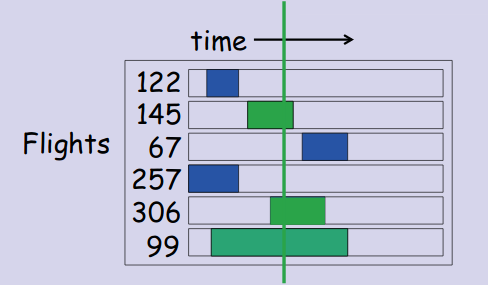
\includegraphics[width=.8\textwidth]{../img/gatetable}
\end{frame}

\begin{frame}
  \frametitle{Problems as Graphs}
  \begin{itemize}
    \item Many problems can be described by the \emph{relationship}
    between the entities in the problem (planes, courses, etc).
    \bigskip

    \item This relationship can be described mathematically using the
    \structure{graph} structure.
  \end{itemize}
\end{frame}

\section{Walks and Paths}
\subsection{Definition}

\begin{frame}
  \frametitle{Directed Graphs (DiGraphs)}

    \begin{columns}
      \column{0.3\textwidth}
      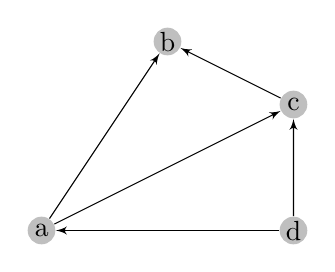
\begin{tikzpicture}[scale=.8,auto,swap]
  \tikzset{edge/.style = {->,>=latex'}}
  \node[vertex] (a) at (0,0) {a};
  \node[vertex] (b) at (2,3) {b};
  \node[vertex] (c) at (4,2) {c};
    \node[vertex] (d) at (4,0) {d};
    \draw[edge] (a) to (b);
    \draw[edge] (a) to (c);
    \draw[edge] (c) to (b);
    \draw[edge] (d) to (c);
    \draw[edge] (d) to (a);
\end{tikzpicture}


      \column{0.7\textwidth}
      A graph is defined by a \structure{set of Vertices} ($V$) and a
      \structure{set of Edges} ($E$). The set of edges is also a
      \structure{relation} from $V$ to $V$.
      \medskip

      \begin{itemize}
        \item $V = \{a,b,c,d\}$
        \item $E = \{(a,b), (a,c), (c,b), (d,c), (d,a)\}$
          \bigskip

          \begin{itemize}
            \item $E: V\rightarrow V$;
            \item $(a,c) \in E$;
            \item $E(a) = c$; \hspace{1cm} \alert{careful!}
            \item $a \rightarrow c$
          \end{itemize}
      \end{itemize}
    \end{columns}
\end{frame}

\begin{frame}
  \frametitle{Relations (Week 2) and Graphs (Week 4)}

  {\larger

  \begin{center}
  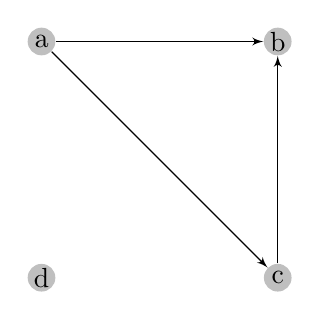
\begin{tikzpicture}[scale=3,auto,swap]
  \tikzset{edge/.style = {->,>=latex'}}
  \node[vertex] (a) at (0,1) {a};
  \node[vertex] (b) at (1,1) {b};
  \node[vertex] (c) at (1,0) {c};
  \node[vertex] (d) at (0,0) {d};
  \draw[edge] (a) to (c);
  \draw[edge] (a) to (b);
  \draw[edge] (c) to (b);
  \end{tikzpicture}\\
  $V = \{a,b,c,d\}$\\
  $E = \{(a,c),(a,b),(c,b)\}$
  \end{center}

  \vfill

  A \structure{digraph with vertices $V$} is the same as a
  \structure{binary relation on $V$}.

  \bigskip

  Every \structure{Binary Relation} can also be written as a directed
  graph!

  }
\end{frame}

\begin{frame}
  \frametitle{Digraphs: Matrix Representation}

  \begin{columns}
    \column{0.5\textwidth}
    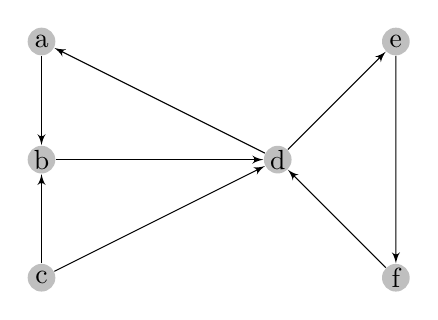
\begin{tikzpicture}[scale=1.5,auto,swap]
      \tikzset{edge/.style = {->,>=latex'}}
      \node[vertex] (a) at (0,1) {a};
      \node[vertex] (b) at (0,0) {b};
      \node[vertex] (c) at (0,-1) {c};
      \node[vertex] (d) at (2,0) {d};
      \node[vertex] (e) at (3,1) {e};
      \node[vertex] (f) at (3,-1) {f};
      \draw[edge] (a) to (b);
      \draw[edge] (c) to (b);
      \draw[edge] (b) to (d);
      \draw[edge] (d) to (a);
      \draw[edge] (c) to (d);
      \draw[edge] (d) to (e);
      \draw[edge] (e) to (f);
      \draw[edge] (f) to (d);
    \end{tikzpicture}
    \column{0.5\textwidth}

    {\larger
      \begin{tabular}{c|cccccc}
        & a & b & c & d & e & f \\
        \hline
        a &0&1&0&0&0&0\\
        b &0&0&0&1&0&0\\
        c &0&1&0&1&0&0\\
        d &1&0&0&0&1&0\\
        e &0&0&0&0&0&1\\
        f &0&0&0&1&0&0\\
      \end{tabular}
    }

    \bigskip

    \begin{center}{\bf Adjacency Matrix}\end{center}
  \end{columns}
  \bigskip

  A value in the adjacency matrix is one if there is an edge between
  the two vertices, 0 otherwise.\\
  \hfill$A(v_i,v_j) = 1$ {\bf iff} $E(v_i) = v_j$
\end{frame}

\subsection{Walks, Paths and Relations}

\begin{frame}
  \frametitle{Walks and Paths}

  There are many properties that we can study in a graph.
  \bigskip

  \begin{itemize}
    \item A {\bf Walk} is a sequence of successive edges;\\

    \bigskip
    \item A {\bf Path} is a walk that does not repeat vertices;\\
  \end{itemize}

\end{frame}

\begin{frame}
  \frametitle{Walk example}

  \begin{center}
    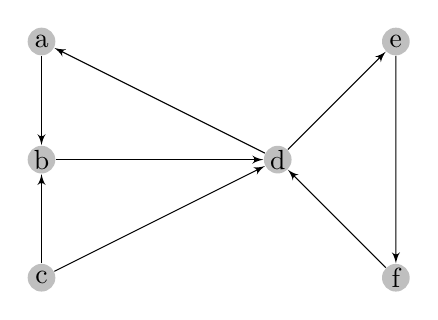
\begin{tikzpicture}[scale=1.5,auto,swap]
      \tikzset{edge/.style = {->,>=latex'}}
      \node[vertex] (a) at (0,1) {a};
      \node[vertex] (b) at (0,0) {b};
      \node[vertex] (c) at (0,-1) {c};
      \node[vertex] (d) at (2,0) {d};
      \node[vertex] (e) at (3,1) {e};
      \node[vertex] (f) at (3,-1) {f};
      \draw[edge] (a) to (b);
      \draw[edge] (c) to (b);
      \draw[edge] (b) to (d);
      \draw[edge] (d) to (a);
      \draw[edge] (c) to (d);
      \draw[edge] (d) to (e);
      \draw[edge] (e) to (f);
      \draw[edge] (f) to (d);
  \end{tikzpicture}
  \end{center}

  \bigskip

  \begin{block}{Walk - sequence of successive edges}

    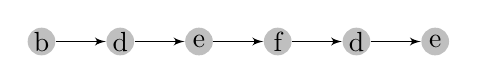
\begin{tikzpicture}[scale=1,auto,swap]
      \tikzset{edge/.style = {->,>=latex'}}
      \node[vertex] (a) at (0,0) {b};
      \node[vertex] (b) at (1,0) {d};
      \node[vertex] (c) at (2,0) {e};
      \node[vertex] (d) at (3,0) {f};
      \node[vertex] (e) at (4,0) {d};
      \node[vertex] (f) at (5,0) {e};
      \draw[edge] (a) to (b);
      \draw[edge] (b) to (c);
      \draw[edge] (c) to (d);
      \draw[edge] (d) to (e);
      \draw[edge] (e) to (f);
    \end{tikzpicture}

    \begin{itemize}
    \item {\bf lengh:} 5 edges (\alert{NOT} 6 vertices)
    \item {\bf as a relation:} $E(E(E(E(E(a)))))$
    \end{itemize}
  \end{block}

\end{frame}

\begin{frame}
  \frametitle{Path example}

  \begin{center}
    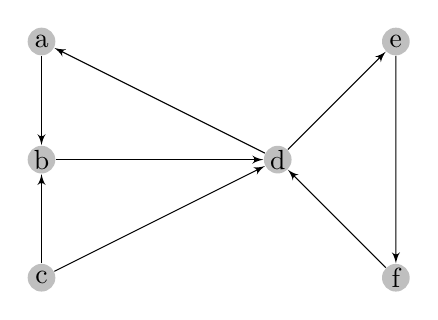
\begin{tikzpicture}[scale=1.5,auto,swap]
      \tikzset{edge/.style = {->,>=latex'}}
      \node[vertex] (a) at (0,1) {a};
      \node[vertex] (b) at (0,0) {b};
      \node[vertex] (c) at (0,-1) {c};
      \node[vertex] (d) at (2,0) {d};
      \node[vertex] (e) at (3,1) {e};
      \node[vertex] (f) at (3,-1) {f};
      \draw[edge] (a) to (b);
      \draw[edge] (c) to (b);
      \draw[edge] (b) to (d);
      \draw[edge] (d) to (a);
      \draw[edge] (c) to (d);
      \draw[edge] (d) to (e);
      \draw[edge] (e) to (f);
      \draw[edge] (f) to (d);
  \end{tikzpicture}
  \end{center}

  \bigskip

  \begin{block}{Path - walk without repeating vertices}

    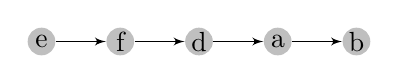
\begin{tikzpicture}[scale=1,auto,swap]
      \tikzset{edge/.style = {->,>=latex'}}
      \node[vertex] (a) at (0,0) {e};
      \node[vertex] (b) at (1,0) {f};
      \node[vertex] (c) at (2,0) {d};
      \node[vertex] (d) at (3,0) {a};
      \node[vertex] (e) at (4,0) {b};
      \draw[edge] (a) to (b);
      \draw[edge] (b) to (c);
      \draw[edge] (c) to (d);
      \draw[edge] (d) to (e);
    \end{tikzpicture}\hspace{1cm} {\bf Stuck!}

    \begin{itemize}
    \item {\bf lengh:} 4 edges
    \item (\alert{NOT} 5 vertices)
    \end{itemize}
  \end{block}
\end{frame}


\subsection{Connectivity}

\begin{frame}
  \frametitle{Walks and Paths: Shortest Path}

  {\larger
    {\bf \structure{Lemma:}} The shortest walk between two vertices is a
    \structure{Path}.
    \begin{enumerate}
    \item {\bf Proof (by contradiction):} Suppose the lemma is not true

      \bigskip

    \item The shortest walk between $v_s$ and $v_e$ is not a path.\\
      $w_s = v_s \rightarrow v_i \rightarrow \ldots \rightarrow v_j \rightarrow v_e$

      \bigskip

    \item This means that this path has at least one repeated vertice, and a walk of size $\geq 1$ between the repetitions.\\
      $w_s = v_s \rightarrow \ldots \rightarrow v_k \rightarrow \ldots \rightarrow v_k \rightarrow \ldots \rightarrow v_e$

      \bigskip

    \item We can create a \structure{new, shorter walk} by removing the edges from $w_s$ between $v_k$ and $v_k$. \alert{Contradiction!}\\
      $w_s' = v_s \rightarrow \ldots \rightarrow v_k \rightarrow \ldots  \rightarrow v_e$
    \end{enumerate}

  }
\end{frame}

\begin{frame}
  \frametitle{The length $n$ walk relation}

    {\huge
  \begin{equation}
    v G^n w
  \end{equation}
    }
  \begin{itemize}
    \item "There is a walk of length $n$ from $v$ to $w$"
    \item $G^n$ is called the \structure{length $n$ walk relation} for G
  \end{itemize}

  \vfill
  \begin{itemize}
  \item $G^1$ is the relation of nodes directly connected by edges.
  \item {\bf lemma:} $G^n \circ G^m = G^{n+m}$
    \hfill (remember that $R\circ S = R(S)$)
  \item $x~G^m \circ G^n~y \rightarrow \exists z, x~G^m~z~G^n~y$
    \hfill ($z \in G^n(y)$ and $x \in G^m(z)$)
  \end{itemize}
\end{frame}

\begin{frame}
  \frametitle{Adjacency Matrices and Composition}

  {\larger
    \begin{itemize}
    \item $A_G$ ::= Adjacency Matrix for \structure{relation $G$}
    \item {\bf lemma:} $A_{G\circ H} = A_G \odot A_H$\\
      where $\odot$ is the \structure{Boolean Matrix Multiplication}
      \bigskip

    \item This allows us to compute $A_{G^n}$ by \structure{Fast
      Matrix Exponentiation}

    \item $A_{G^n} = A_{G^{n/2}} \odot A_{G^{n/2}} = \ldots$

      \end{itemize}
  }
\end{frame}

\begin{frame}
  \frametitle{Walk Relation of a DiGraph}

  \begin{itemize}
  \item $G^*$ is the \structure{walk relation} of $G$
  \item $u G^* v$ {\bf iff} $\exists$ walk from $u$ to $v$
    \structure{of any length}\\
  \end{itemize}

  \vfill
  How do we calculate calculte $G^*$? Walks can be infinite,
  so is there a {\bf finite} algorithm to calculate it?
\end{frame}

\begin{frame}
  \frametitle{Walk Relation of a DiGraph}

  Algorithm to calculate $G^*$:
  \begin{itemize}
  \item Add self loops to the graph:
    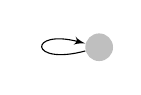
\begin{tikzpicture}[scale=1.5,auto,swap]
      \tikzset{edge/.style = {->,>=latex'}}
      \node[vertex] (a) at (0,0) {};
      \draw[edge] (a) to[loop left] (a);
    \end{tikzpicture}
  \item This is equivalent to defining $G^{\leq} = G \cup G^0$
  \item $G^{\leq}$ has a walk length $n$ {\bf iff}
    $G$ has a walk of length $\leq n$
  \item $G^* = (G^{\leq})^{n-1}$\\
  \end{itemize}
  \vfill

  \alert{QUIZ: Why is it necessary to add the self-loop?}
\end{frame}

\section{Scheduling and Partial Orders}
\subsection{Directed Acyclic Graphs (DAGs)}

\begin{frame}
  \frametitle{Applications of Walks: Prerequisite Trees}
  \begin{center}
    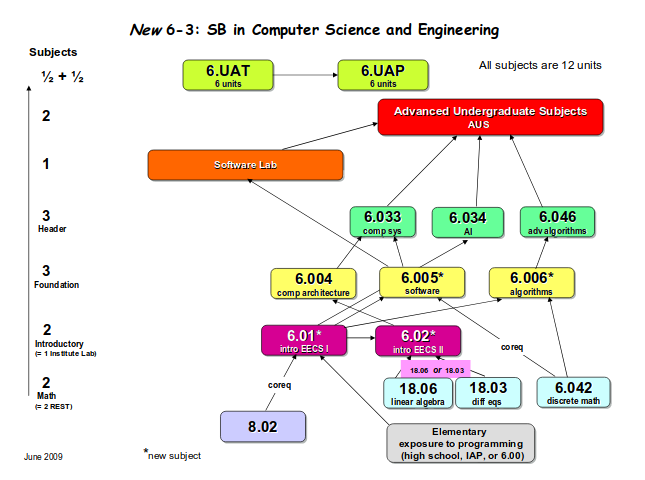
\includegraphics[width=0.8\textwidth]{../img/MIT_prereq}
  \end{center}
\end{frame}

\begin{frame}
  \frametitle{Prerequisite Trees}
  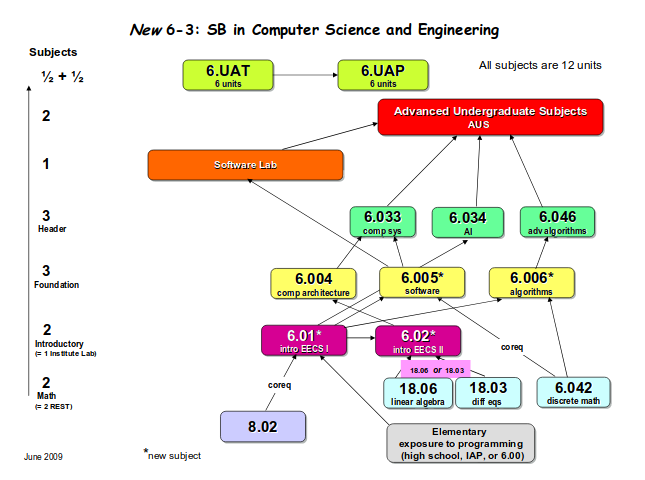
\includegraphics[width=0.2\textwidth]{../img/MIT_prereq}

  {\larger
    \begin{itemize}
    \item \structure{Direct Prerequisite}: Req(6.046) = 6.006
    \item \structure{Indirect Prerequisite}: Req(6.046) = $\{6.006, 6.042, 6.01, 6.00, 8.02\}$
    \end{itemize}

    \vfill

    u is an indirect prerequisite of v means that:

    \bigskip

    \begin{center}
      There is \structure{a positive length walk} from $u$ to $v$ in
      graph D.
      \begin{equation*}
        u D^+ v
      \end{equation*}
    \end{center}
  }
\end{frame}

\begin{frame}
  \frametitle{Requisites, Cycles and DAGs}

  {\large
    \begin{itemize}
    \item A \structure{closed walk} is a walk that starts and ends at
      the same vertex.\\
      \begin{center}
        {\bf Q:} How long does it take to graduate if there is a
        closed walk in the prerequisite graph?
      \end{center}

      \bigskip

    \item A \structure{cycle} is a closed walk where the only repeat
      vertex is at the beginning and end.\\
      $v_0 \rightarrow v_1 \rightarrow \ldots \rightarrow v_n-1 \rightarrow v_0 | v_{i > 0}$ does not repeat.
      \begin{itemize}
        \item {\bf OR} A cycle is a path from $v \rightarrow w + (w,v) \in E$
      \end{itemize}
      \bigskip

    \item A \alert{Directed Acyclic Graph (DAG)} is a digraph that has
      \structure{no positive length cycles}.
    \end{itemize}

  }
\end{frame}

\begin{frame}
  \frametitle{DAG Examples}

    \begin{itemize}
      \item Class Prerequisite Graphs;
      \item Ordered Task List:\\
        ``first add rice, then add water, then press cook button''
        \bigskip
    \end{itemize}
    \bigskip

    Some weird things can be described as DAGs:
    \bigskip

    \begin{itemize}
      \item The \structure{Successor Relation}:
        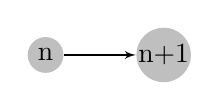
\begin{tikzpicture}[scale=1.5,auto,swap]
          \tikzset{edge/.style = {->,>=latex'}}
          \node[vertex] (a) at (0,0) {$\text{  n  }$};
          \node[vertex] (b) at (1,0) {n+1};
          \draw[edge] (a) to (b);
        \end{tikzpicture}, $a < b$

        \bigskip

      \item The \structure{Subset Relation $\subset$}: $\{1,2\} \subset
        \{1,2,3\}$
      \item Dynamic Programming;
      \item Induction Proofs;
    \end{itemize}
\end{frame}

\begin{frame}
  \frametitle{DAG Walk Relation}

  \begin{columns}
    \column{0.3\textwidth}
    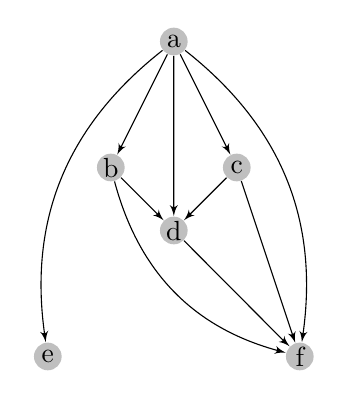
\begin{tikzpicture}[scale=.8,auto,swap]
      \tikzset{edge/.style = {->,>=latex'}}
      \node[vertex] (a) at (2,5) {a};
      \node[vertex] (b) at (1,3) {b};
      \node[vertex] (c) at (3,3) {c};
      \node[vertex] (d) at (2,2) {d};
      \node[vertex] (e) at (0,0) {e};
      \node[vertex] (f) at (4,0) {f};
      \draw[edge] (a) to (b);
      \draw[edge] (a) to (c);
      \draw[edge] (a) to (d);
      \draw[edge] (c) to (f);
      \draw[edge] (d) to (f);
      \draw[edge] (c) to (d);
      \draw[edge] (b) to (d);
      \draw[edge] (a) to[bend right] (e);
      \draw[edge] (a) to[bend left] (f);
      \draw[edge] (b) to[bend right] (f);
    \end{tikzpicture}
    \column{0.7\textwidth}

    {\larger
      Given a DAG $A$, what is the \structure{smallest} DAG $B$ with
      the same \structure{Walk Relation}?
      \begin{itemize}
      \item $a\rightarrow e$
      \item $a\rightarrow c\rightarrow f$
      \item $a\rightarrow b\rightarrow d\rightarrow f$
      \end{itemize}

      \hfill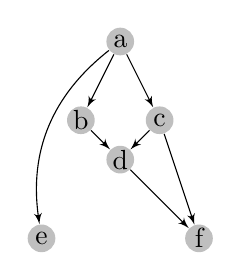
\begin{tikzpicture}[scale=.5,auto,swap]
        \tikzset{edge/.style = {->,>=latex'}}
        \node[vertex] (a) at (2,5) {a};
        \node[vertex] (b) at (1,3) {b};
        \node[vertex] (c) at (3,3) {c};
        \node[vertex] (d) at (2,2) {d};
        \node[vertex] (e) at (0,0) {e};
        \node[vertex] (f) at (4,0) {f};
        \draw[edge] (a) to (b);
        \draw[edge] (a) to (c);
        \draw[edge] (c) to (f);
        \draw[edge] (d) to (f);
        \draw[edge] (c) to (d);
        \draw[edge] (b) to (d);
        \draw[edge] (a) to[bend right] (e);
      \end{tikzpicture}\\
      \hfill B is the \structure{Covering Edges} of DAG A;
    }
  \end{columns}
\end{frame}

\subsection{Scheduling}

\begin{frame}
  \frametitle{Using DAGs for Scheduling}

  \begin{columns}[T]
    \column{0.3\textwidth}
    $18.01 \rightarrow 6.042$\\
    $18.01 \rightarrow 18.02$\\
    $18.01 \rightarrow 18.03$
    \column{0.35\textwidth}
    $6.001 \rightarrow 6.034$\\
    $6.042 \rightarrow 6.046$\\
    $8.02 \rightarrow 6.002$\\
    $18.03, 6.002 \rightarrow 6.004$
    \column{0.35\textwidth}
    $6.001, 6.004 \rightarrow 6.033$\\
    $6.033 \rightarrow 6.857$\\
    $6.046 \rightarrow 6.840$
  \end{columns}

  \vfill

  {\larger

    $u$ is a \structure{indirect prerequisite} of $v$ if there is a
    posiive length walk in graph $R$: $u R^+ v$

    \begin{center}
      $18.01 \rightarrow 6.042 \rightarrow 6.046 \rightarrow 6.840$
    \end{center}

  }
\end{frame}

\begin{frame}
  \frametitle{Scheduling: Minimal Subject}

  {\larger
    \begin{itemize}
    \item A \structure{minimal} subject is does not have any prerequisites.
      \begin{center}
        nothing $\rightarrow 18.01$, nothing $\rightarrow 6.001$, nothing $\rightarrow 8.02$
      \end{center}

      \bigskip

    \item A \structure{minimum} subject comes before all other
      subjects. {\bf Indirect Prerequisite of all subjects!}
      \begin{center}
        none in this example...
      \end{center}
      \bigskip

    \item \structure{Maximal} and \structure{Maximum} subjects have
      similar definition. \alert{QUIZ:} What is a Maximum subject?

    \end{itemize}
  }
\end{frame}

\begin{frame}
  \frametitle{Scheduling}

  \begin{columns}[T]
    \column{0.3\textwidth}
    $18.01 \rightarrow 6.042$\\
    $18.01 \rightarrow 18.02$\\
    $18.01 \rightarrow 18.03$
    \column{0.35\textwidth}
    $6.001 \rightarrow 6.034$\\
    $6.042 \rightarrow 6.046$\\
    $8.02 \rightarrow 6.002$\\
    $18.03, 6.002 \rightarrow 6.004$
    \column{0.35\textwidth}
    $6.001, 6.004 \rightarrow 6.033$\\
    $6.033 \rightarrow 6.857$\\
    $6.046 \rightarrow 6.840$
  \end{columns}

  \vfill

  {\larger
    Greedy Scheduling:
    \begin{enumerate}
    \item Identify Minimal Subjects;
    \item Add Minimal Subjects to Schedule;
    \item Remove Minimal Subjects;
    \item Return to Step 1
    \end{enumerate}
  }
\end{frame}

\begin{frame}
  \frametitle{Greedy Scheduling}
  \begin{center}
    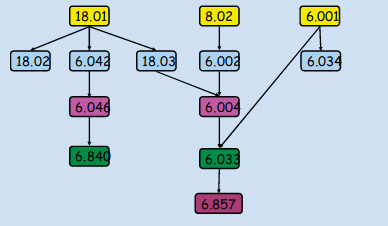
\includegraphics[width=0.8\textwidth]{../img/greedy_schedule}
  \end{center}
\end{frame}

\begin{frame}
  \frametitle{Anti-Chains}
  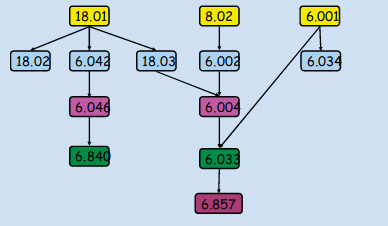
\includegraphics[width=0.5\textwidth]{../img/greedy_schedule}

  {\larger
    \begin{itemize}
    \item An \structure{anti-chain} is a set of subjects which does
      not include \structure{indirect requisites}
    \item The subjects in an anti-chain can be \structure{taken in any
      order}
    \item They are also called \structure{incomparable} (no path)
      \medskip
      \begin{center}
        Example: $\{6.046, 6.004\},\{6.001, 6.002, 6.046, 18.02\}$
      \end{center}
    \end{itemize}
  }
\end{frame}

\begin{frame}
  \frametitle{A Lazy Scheduling}

  {\larger
  \begin{itemize}
  \item Can we take only 1 subject per term?\\

    \begin{center}
      18.01, 6.001, 8.02, 6.002, 18.03, 6.034, 6.042, 18.02, 6.004,
      6.046, 6.033, 6.840, 6.857
    \end{center}

    \bigskip

  \item This is called a ``topological sort''.

    \bigskip

  \item A \structure{chain} is a set of subjects which all have a
    \structure{prerequisite relation} to each other.

    \bigskip

  \item It is possible to show that the \structure{maximum chain} is
    the requisite and necessary numbers of terms to finish a program.

  \end{itemize}
  }
\end{frame}

\subsection{Scheduling and Processors}

\begin{frame}
  \frametitle{Parallel Processing}

  {\larger
    \begin{itemize}
    \item The schedule of courses in terms is an example of the more general idea of \structure{parallel scheduling}

      {\large
        \begin{itemize}
        \item \structure{minimum terms to graduate}: Minimal parallel
          time (assuming no limit on parallel tasks)
        \item Minimal Parallel Time = Max Chain Size
        \item \structure{maximum term load}: Number of processors
          needed;
        \item Processors for minimum time $\leq$ maximum anti-chain
          size.
        \end{itemize}
      }

      \vfill

    \item Minimum Load with $n$ tasks and $m$ max chain size:

      \begin{equation}
        \text{min. load} \geq \lceil n/m  \rceil
      \end{equation}
    \end{itemize}
  }

\end{frame}

\section{Partial Orders and Equivalence}

\begin{frame}
  \frametitle{Walks and transitivity}

  {\larger

    \begin{itemize}
    \item If there is a walk from $u$ to $v$, and a walk from $v$ to $w$
    \item This implies there is a walk from $u$ to $w$
    \end{itemize}
    \begin{center}
      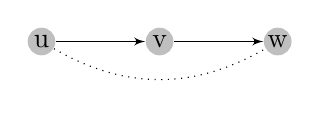
\begin{tikzpicture}[scale=.5,auto,swap]
        \tikzset{edge/.style = {->,>=latex'}}
        \node[vertex] (a) at (0,0) {u};
        \node[vertex] (b) at (3,0) {v};
        \node[vertex] (c) at (6,0) {w};
        \draw[edge] (a) to (b);
        \draw[edge] (b) to (c);
        \draw[dotted] (a) to[bend right] (c);
      \end{tikzpicture}
    \end{center}
    Expressing this idea as a \structure{walk relation} in G:
    \begin{equation}
      uG^+v \land vG^+w \implies uG^+w
    \end{equation}

    \vfill
    \begin{block}{Transitivity in Relations}
      Any relation {\bf R} is transitive if:
      $xRy \land yRz \implies xRz$
    \end{block}
  }
\end{frame}

\begin{frame}
  \frametitle{DAG and assimetry}

  {\larger

    In an \structure{Acyclic Graph D} we can see that
    \begin{itemize}
    \item A positive length path from $u$ to $v$ implies no
      path from $v$ to $u$;

      \bigskip

    \item $uD^+v \implies \text{NOT}(vD^+u)$

      \bigskip

    \item \structure{Property of Assimetry} or Assimetry Relation R
    \end{itemize}
  }
\end{frame}

\begin{frame}
  \frametitle{Strict Partial Order}

  {\larger

    A relation $R$ is a \structure{Strict Partial Order} {\bf iff} it
    is {\bf Transitive} and {\bf Assimetric}.

    \bigskip

    Examples:
    \begin{itemize}
    \item The $\subset$ relation on sets
    \item The ``indirect prerequisite'' relationship on subjects.
    \item The $<$ relationship on $\mathbb{R}$
    \end{itemize}

    \bigskip

    R is an \structure{SPO} {\bf iff} $R = D^+$ for some DAG $D$.
  }
\end{frame}

\begin{frame}
  \frametitle{Path Total Orders}

  {\larger
    A \structure{partial order} is also \structure{Path Total} if for
    any two distinct elements, one will be ``greater than'' another.

    \bigskip

    Example: $<$ or $\leq$ on $\mathbb{R}$: if $x,y \in \mathbb{R},
    x\neq y \implies x>y \text{ or } y>x$

    \bigskip

    Counter-Example: $\subset$ in POW($\mathbb{N}$): $\{1,3\} \not\subset \{2,5\} \not\subset \{1,3\}$

    \vfill

    \begin{itemize}
    \item Relation $R$ is \structure{path total}: if $x \neq y \implies xRy \lor yRx$
    \item This means there are \alert{no imcomparable elements}
    \end{itemize}
  }
\end{frame}

\begin{frame}
  \frametitle{Path totality}

  {\larger

    In a \structure{path total} relation, the whole graph is a
    \structure{chain}
  \begin{center}
    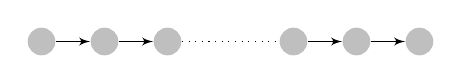
\begin{tikzpicture}[scale=.8,auto,swap]
      \tikzset{edge/.style = {->,>=latex'}}
      \node[vertex] (a) at (0,0) {};
      \node[vertex] (b) at (1,0) {};
      \node[vertex] (c) at (2,0) {};
      \node[vertex] (d) at (4,0) {};
      \node[vertex] (e) at (5,0) {};
      \node[vertex] (f) at (6,0) {};
      \draw[edge] (a) to (b);
      \draw[edge] (b) to (c);
      \draw[dotted] (c) to (d);
      \draw[edge] (d) to (e);
      \draw[edge] (e) to (f);
    \end{tikzpicture}
  \end{center}

  \bigskip

  A \structure{weak partial order} is the same as a \structure{strict
    partial order} R, except that $aRa$ always holds:
  \begin{center}
    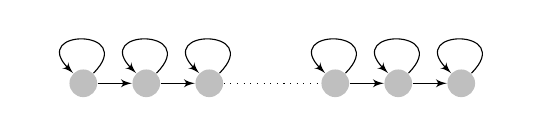
\begin{tikzpicture}[scale=.8,auto,swap]
      \tikzset{edge/.style = {->,>=latex'}}
      \node[vertex] (a) at (0,0) {};
      \node[vertex] (b) at (1,0) {};
      \node[vertex] (c) at (2,0) {};
      \node[vertex] (d) at (4,0) {};
      \node[vertex] (e) at (5,0) {};
      \node[vertex] (f) at (6,0) {};
      \draw[edge] (a) to (b);
      \draw[edge] (b) to (c);
      \draw[dotted] (c) to (d);
      \draw[edge] (d) to (e);
      \draw[edge] (e) to (f);
      \draw[edge] (a) to[loop] (a);
      \draw[edge] (b) to[loop] (b);
      \draw[edge] (c) to[loop] (c);
      \draw[edge] (d) to[loop] (d);
      \draw[edge] (e) to[loop] (e);
      \draw[edge] (f) to[loop] (f);
    \end{tikzpicture}
  \end{center}

  \bigskip

  \begin{itemize}
  \item Examples: $\subseteq$ on sets, $\leq$ on $\mathbb{R}$
  \item Weak Partial Orders define the property of
    \structure{Reflexivity}
  \item Relation $R$ on $A$ is \structure{reflexive} {\bf iff} $aRa,
    \forall a\in A$
  \end{itemize}

  }
\end{frame}

\begin{frame}
  \frametitle{Assimetry and Antissimetry}

  {\larger

    \begin{block}{Assimetry}
      \begin{itemize}
      \item Reflexibility is \alert{never} allowed
      \item R is \structure{assimetric} {\bf iff}:
        \begin{equation}
          xRy \implies \text{NOT}(yRx)
        \end{equation}
      \end{itemize}

    \end{block}

    \begin{block}{Antissimetry}
      \begin{itemize}
      \item Reflexibility is \alert{sometimes} allowed
      \item R is \structure{antissimetric} {\bf iff}
        \begin{equation}
          xRy \implies \text{NOT}(yRx), \text{ for } x \neq y
        \end{equation}
      \end{itemize}
    \end{block}
  }
\end{frame}

\begin{frame}
  \frametitle{Definition of Weak Partial Order}

  {\huge

    $R$ is a WPO {\bf iff}\\ $R = D^*$ for some DAG $D$
  }
\end{frame}

\subsection{Partial Orders and Subset Relations}
\begin{frame}
  \frametitle{Proper Subset Relation}

  \begin{itemize}
  \item $A\subset B$ means that \structure{B has everything A has},
    and \alert{something extra} ($B \not\subset A$)

    \bigskip

  \item Example of proper subset relation:
\begin{center}
    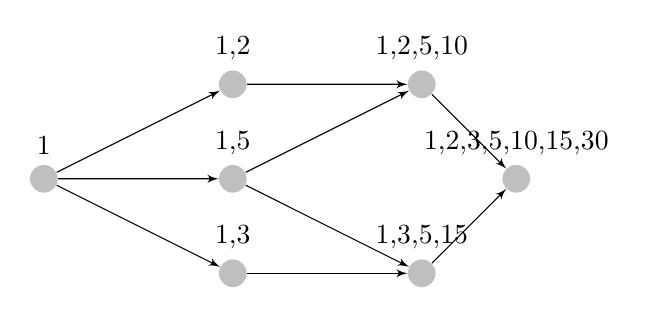
\begin{tikzpicture}[scale=1.2,auto,swap]
      \tikzset{edge/.style = {->,>=latex'}}
      \node[vertex,label={1}] (a) at (0,1) {};
      \node[vertex,label={1,3}] (b) at (2,0) {};
      \node[vertex,label={1,5}] (c) at (2,1) {};
      \node[vertex,label={1,2}] (d) at (2,2) {};
      \node[vertex,label={1,3,5,15}] (e) at (4,0) {};
      \node[vertex,label={1,2,5,10}] (f) at (4,2) {};
      \node[vertex,label={1,2,3,5,10,15,30}] (g) at (5,1) {};
      \draw[edge] (a) to (b);
      \draw[edge] (a) to (c);
      \draw[edge] (a) to (d);
      \draw[edge] (c) to (e);
      \draw[edge] (b) to (e);
      \draw[edge] (c) to (f);
      \draw[edge] (d) to (f);
      \draw[edge] (e) to (g);
      \draw[edge] (f) to (g);
    \end{tikzpicture}
  \end{center}

  \end{itemize}
\end{frame}

\begin{frame}
  \frametitle{Partial Order: Proper Divides}

  {\larger
    \begin{itemize}
    \item a \structure{proper divides} b if $a|b$ and $a \neq b$
      \begin{center}
        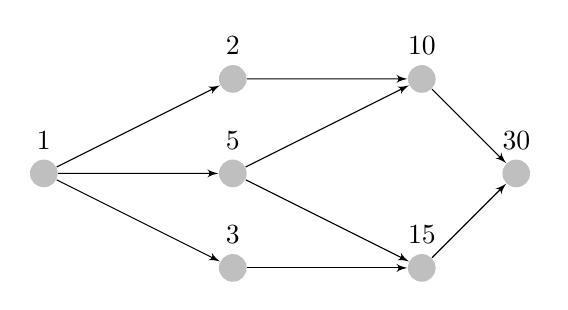
\begin{tikzpicture}[scale=1.2,auto,swap]
          \tikzset{edge/.style = {->,>=latex'}}
          \node[vertex,label={1}] (a) at (0,1) {};
          \node[vertex,label={3}] (b) at (2,0) {};
          \node[vertex,label={5}] (c) at (2,1) {};
          \node[vertex,label={2}] (d) at (2,2) {};
          \node[vertex,label={15}] (e) at (4,0) {};
          \node[vertex,label={10}] (f) at (4,2) {};
          \node[vertex,label={30}] (g) at (5,1) {};
          \draw[edge] (a) to (b);
          \draw[edge] (a) to (c);
          \draw[edge] (a) to (d);
          \draw[edge] (c) to (e);
          \draw[edge] (b) to (e);
          \draw[edge] (c) to (f);
          \draw[edge] (d) to (f);
          \draw[edge] (e) to (g);
          \draw[edge] (f) to (g);
        \end{tikzpicture}
      \end{center}

      \bigskip

    \item The \structure{proper divide} relation has {\bf the same
      shape} as the $\subset$ relation.

    \item Both relations are \alert{isomorphic}.

    \end{itemize}
  }
\end{frame}

\begin{frame}
  \frametitle{Isomorphism}

  {\larger

    \begin{itemize}
    \item Two graphs are \structure{isomorphic} if they have the same
      \structure{connections}

      \bigskip

    \item More formally, two graphs are \structure{isomorphic} if
      there is a \structure{edge preserve matching (bijection)}
      between their vertices.

      \bigskip

    \item $G_1 \text{ isomorphic } G_2 \iff \exists \text { bijection
    } f:V_1\rightarrow V_2$\\\hfill with $(u,v) \in E_1 \iff
      (f(u),f(v)) \in E_2$

    \end{itemize}
  }
\end{frame}

\begin{frame}
  \frametitle{Isomorphism, $\subset$ and partial orders}

  {\larger
    {\bf Theorem:} Every strict p.o. $R$ is isomorphic to some
    collection of sets partially ordered by $\subset$.

    \bigskip

    {\bf Proof (by construction):}
    \begin{itemize}
    \item Map element $a$ to the set of elements below it.
    \item in other words, $a$ maps to $\{b \in A| bRa \lor b = a\}$\\
      \hfill(remember that NOT$(aRa)$)
    \item in other words, $f(a) ::= R^{-1}(a) \cup \{a\}$
    \end{itemize}

    \bigskip

    {\bf Example:} from divides
    \begin{itemize}
    \item $f(10) = 1|10, 2|10, 5|10, \cup \{10\} = \{1,2,5,10\}$
    \item $f(3) = 1|3, \cup \{3\} = \{1,3\}$
    \end{itemize}
  }
\end{frame}

\subsection{Equivalence Relations}

\begin{frame}
  \frametitle{Symmetric Relations and Equivalence Relations}

  {\larger
    \begin{itemize}
    \item If there is a walk from $u$ to $v$ and a walk from $v$ to
      $u$, then we say that $u$ and $v$ are \structure{strongly
      connected}.\\
      $uG^*v$ and $vG^*u$

      \bigskip

    \item Relation $R$ is \structure{symmetric} if $aRb \implies bRa$. The \structure{strongly connected} relation is symmetric.

      \bigskip

    \item An \structure{equivalence relation} $R$ is: transitive,
      symmetric and reflexive.

      \bigskip

    \item R is an \structure{equivalence relation} {\bf iff} $R$ is
      the \structure{strongly connected} relation of some DiGraph.

    \end{itemize}
  }
\end{frame}

\begin{frame}
  \frametitle{Equivalence Relations Examples}

  {\larger
    Examples:
    \begin{itemize}
    \item Equality: $=$
    \item $\equiv $(mod n)
    \item Same Size, Same Color, etc.
    \end{itemize}

  }
\end{frame}

\begin{frame}
  \frametitle{Relation Properties: Graphical Review}

  {\larger

    \begin{columns}
      \column{0.5\textwidth}
      \begin{center}
      Reflexive:\\
      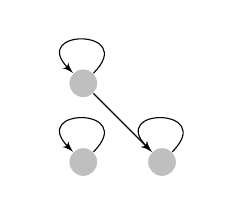
\begin{tikzpicture}[scale=1,auto,swap]
        \tikzset{edge/.style = {->,>=latex'}}
        \node[vertex] (a) at (0,0) {};
        \node[vertex] (b) at (1,0) {};
        \node[vertex] (c) at (0,1) {};
        \draw[edge] (a) to[loop] (a);
        \draw[edge] (b) to[loop](b);
        \draw[edge] (c) to[loop] (c);
        \draw[edge] (c) to (b);
      \end{tikzpicture}

      \bigskip

      Transitive:\\
      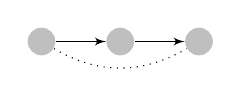
\begin{tikzpicture}[scale=1,auto,swap]
        \tikzset{edge/.style = {->,>=latex'}}
        \node[vertex] (a) at (0,0) {};
        \node[vertex] (b) at (1,0) {};
        \node[vertex] (c) at (2,0) {};
        \draw[edge] (a) to (b);
        \draw[edge] (b) to (c);
        \draw[dotted] (a) to[bend right] (c);
      \end{tikzpicture}
      \end{center}
      \column{0.5\textwidth}
      \begin{center}
      Assymetric:\\
      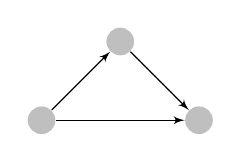
\begin{tikzpicture}[scale=1,auto,swap]
        \tikzset{edge/.style = {->,>=latex'}}
        \node[vertex] (a) at (0,0) {};
        \node[vertex] (b) at (1,1) {};
        \node[vertex] (c) at (2,0) {};
        \draw[edge] (a) to (b);
        \draw[edge] (b) to (c);
        \draw[edge] (a) to (c);
      \end{tikzpicture}

      \bigskip

      Symetric:\\
      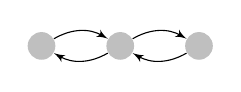
\begin{tikzpicture}[scale=1,auto,swap]
        \tikzset{edge/.style = {->,>=latex'}}
        \node[vertex] (a) at (0,0) {};
        \node[vertex] (b) at (1,0) {};
        \node[vertex] (c) at (2,0) {};
        \draw[edge] (a) to[bend left] (b);
        \draw[edge] (b) to[bend left] (a);
        \draw[edge] (b) to[bend left] (c);
        \draw[edge] (c) to[bend left] (b);
      \end{tikzpicture}

      \end{center}
    \end{columns}
  }
\end{frame}

\begin{frame}
  \frametitle{Representing Equivalence}
  {\larger

    \begin{itemize}
    \item For a total function $f:A\rightarrow B$
    \item We can define an equivalence relation: $\equiv_f$ on $A$:
      \begin{equation}
        a \equiv_f a' \iff f(a) = f(a')
      \end{equation}

      \bigskip

    \item {\bf Theorem:} Relation $R$ on set $A$ is an equiv. relation
      {\bf iff}: $R$ is $\equiv_f$ for some $f:A\rightarrow B$

      \bigskip

    \item {\bf Example:} $\equiv$ (mod n) is $\equiv_f$
      \structure{where} $f(k) ::= \text{rem}(k,n)$
    \end{itemize}
  }
\end{frame}

\begin{frame}
  \frametitle{Equivalence and Partition}

  {\larger
    \begin{itemize}
    \item We define a \structure{partition} $\Pi$ of a set $A$, where
      $\$Pi$ is a collection of subsets of $A$ that cover all elements
      but do not overlap.

      \bigskip

      {\bf Example:} For A = $\{a,b,c,d,e\}$ one partition could be:
      $\{a,b\},\{c,e\},\{d\}$


      \bigskip

    \item We define a relatin $\equiv_{\Pi}$ on A: $a \equiv_{\Pi} a'$
      if both $a$ and $a'$ are in the same subset of $\Pi$

      \bigskip

    \item A relation $R$ on set $A$ is an equivalence relation {\bf
      iff} $R$ is $\equiv_{\Pi}$ for some partition $\Pi$ of $A$.
    \end{itemize}

  }
\end{frame}


\section{Degrees and Isomorphism}

\section{Conclusion}
\begin{frame}
  \frametitle{Lecture Summary}

  {\larger
  \begin{itemize}
  \item Graphs can be seen as relations on vertices;
  \item Vertex connectivity by n-1 power of adjacency matrix;
  \item DAG have no cycles, and define {\bf order} relationships;
  \item Properties of Relations: Symmetry, Transitivity, Reflexivity;
  \item Equivalence relations;
  \end{itemize}
  }
\end{frame}
\end{document}
